\chapter{Eredmények}
\pagestyle{headings}


\section{Sejtekből kiszabaduló káliumion koncentráció közelítő számítása}
A kísérletes munkát megelőzően számolásokat végeztem el annak érdekében, hogy az elektród képes lesz detektálni a sejt szétesést követően az intracelluláris térből felszabaduló kálium-ion mennyiséget., hiszen, mint minden készülékkel, így a kálium- ionszelektív elektróddal is csak meghatározott tartományon belül lehet pontos mérést végezni. Az elektród alsó kimutatási határa 10$^{-6}$, 10$^{-6}$ M. 
 A számolás lépései a következőek voltak: 
Megnéztem az általam vizsgálandó fajra \emph{Candida albicans} jellemző sejttérfogatot \cite{chaffin1984relationship}, ami körülbelül $\upmu m^3$/. Kiszámoltam, hogy 10 cm$^3$  oldatban mennyi a teljes intracelluláris térfogat, ha a sejtkoncentráció 1cm$^3$ térfogatban 10$^7$ db sejt. Viszont szükséges volt annak a meghatározása is, ha az összes sejt szétesik, akkor mennyi lesz az összes felszabadult káliumion koncentráció. Az intracelluláris kálium-ionkoncentráció (0.1 M) és a teljes intracelluláris térfogat(2 $\cdot$ 10$^9$ $\upmu m^3$) szorzatából kiszámoltam 2 $\cdot$ 10$^{-6}$ $dm^3$ sejttérfogatban lévő teljes kálium-ion anyagmennyiséget (2 $\cdot$ 10$^{-7}$ mol), majd ezt elosztottam az oldat (0.01 $dm^3$) térfogatával, így megkaptam a teljes extracelluláris kálium-ionkoncentrációt (2 $\cdot$ 10$^{-5}$ M) arra vonatkozóan, ha az összes sejt károsodást szenvedne. A kapott eredmények alapján elmondható, hogy elvégezhető a mérés, mert a számolt kálium-ionkoncentráció nagyobb, mint a legkisebb koncentráció, amit az elektród még képes detektálni/kimutatni. 

\section{Káliumion szelektív elektródok kalibrációja}
A méréshez használt elektródokon kalibrációt végeztem el, hogy a kapott egyenes egyenletének segítségével a potenciálértékekből tudjak koncentrációt számolni. A jobb nyomon követhetőség és érthetőség érdekében bizonyos lépéseket újból leírok.



10$^7$ db sejt/cm$^3$ $\cdot$ 10 cm$^3$ = 10$^8$ db sejt

10$^8$ db sejt $\cdot$ 20 $\upmu m^3$/sejt = 2 $\cdot$ 10$^9$ $\upmu m^3$ = 2 $\cdot$ 10$^{-6}$ $dm^3$

ha az összes sejt szétesik, és az összes intracelluláris káliumion kiszabadul az extracelluláris térbe:

2 $\cdot$ 10$^{-6}$ $dm^3$ $\cdot$ 0.1 M = 2 $\cdot$ 10$^{-7}$ mol

2 $\cdot$ 10$^{-7}$ mol / 0.01 $dm^3$ = 2 $\cdot$ 10$^{-5}$ M


\section{Káliumion kiáramlás nyomon követése ionszelektív elektróddal}

\begin{figure}
\centering
\includegraphics[width=0.7\textwidth, angle=-90]{img/meres.eps}
\caption{képaláírás}
\label{fig:mérések}
\end{figure}

Ahogy az a \ref{fig:mérések}. ábrán látható.


